\begin{figure}[!t]
\begin{subfigure}{\linewidth}
\centering
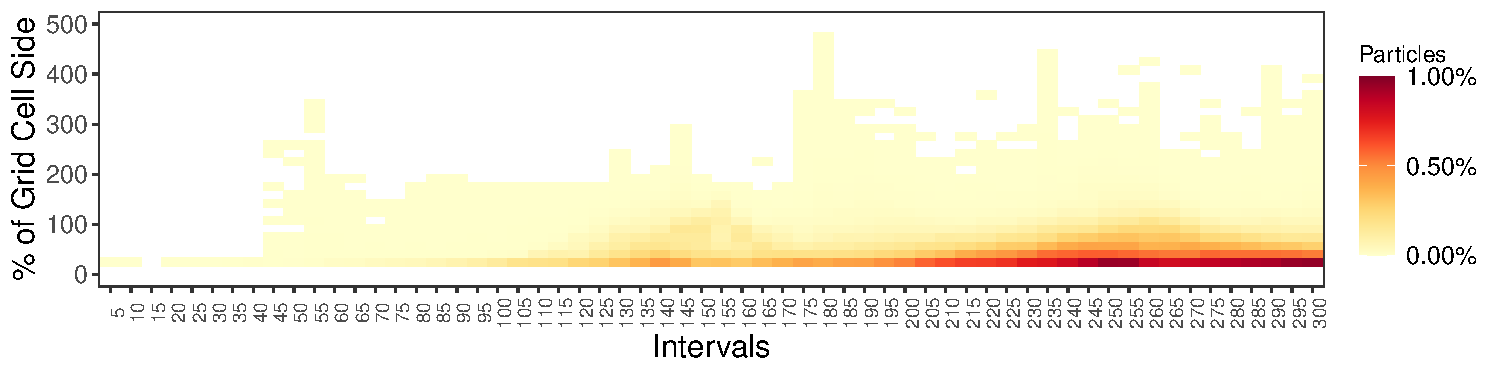
\includegraphics[width=\linewidth]{Images/Jet_Intervals_T1_Percent.pdf}
\caption{T1, 1:1}
\label{fig:jet_1}
\end{subfigure}
\begin{subfigure}{\linewidth}
\centering
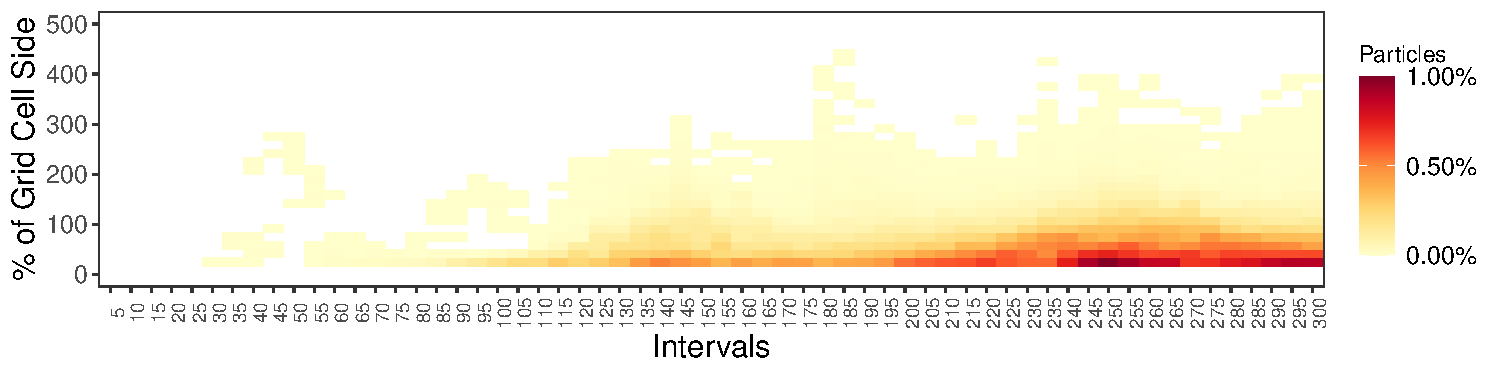
\includegraphics[width=\linewidth]{Images/Jet_Intervals_T3_Percent.pdf}
\caption{T3, 1:8}
\label{fig:jet_3}
\end{subfigure}
\begin{subfigure}{\linewidth}
\centering
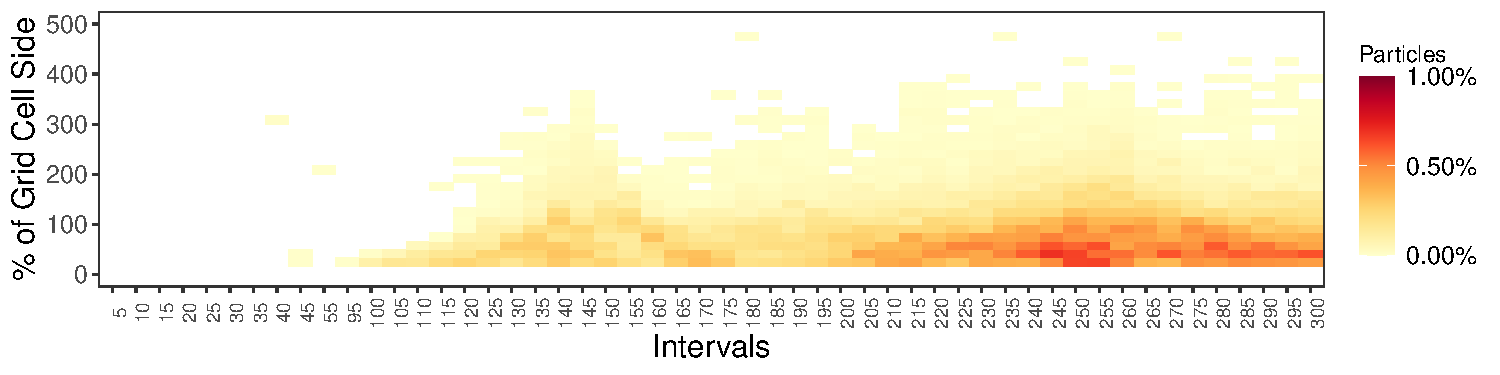
\includegraphics[width=\linewidth]{Images/Jet_Intervals_T5_Percent.pdf}
\caption{T5, 1:27}
\label{fig:jet_5}
\end{subfigure}
\begin{subfigure}{\linewidth}
\centering
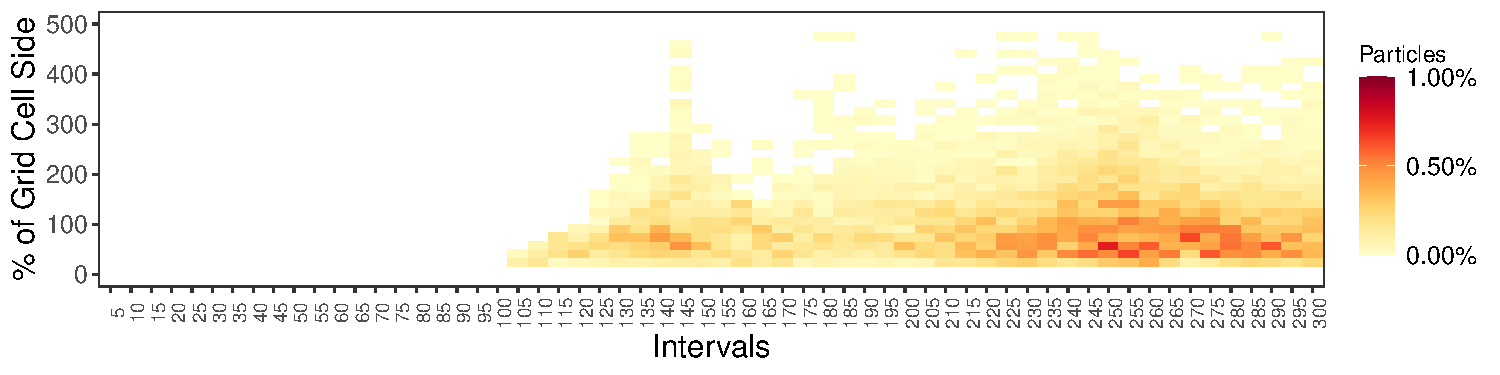
\includegraphics[width=\linewidth]{Images/Jet_Intervals_T7_Percent.pdf}
\caption{T7, 1:64}
\label{fig:jet_7}
\end{subfigure}
\caption{Jet tests showing the impact of variation in the data reduction factor on the distribution of reconstruction error.}
\label{fig:jet_map}
\end{figure}
